% canary-signal-flow.tex  v2  (OMN-175)
% End-to-end RayaChain canary signal flow
% 4 swimlanes: Detect / Transform / Propagate / Decide+Respond
% 13 activities (A1-A13), 3 decision diamonds, L1/L2 honesty marker,
% audit sub-rail, feedback loop A13->A4
%
% Compile:  pdflatex canary-signal-flow.tex
% Include in IEEEtran two-column:
%   \begin{figure*}
%     \centering
%     
\includegraphics[width=\textwidth]{figures/canary-signal-flow}
%     \caption{...}
%   \end{figure*}

\documentclass{article}
\usepackage[margin=0pt]{geometry}
\pagestyle{empty}
\usepackage[T1]{fontenc}
\usepackage{lmodern}
\usepackage{amsmath}
\usepackage{tikz}
\usetikzlibrary{arrows.meta,shapes.geometric,backgrounds,calc}

\definecolor{layerblue}{RGB}{90,130,175}  %% muted blue: L1/L2 distinction only

\newsavebox{\figbox}

\begin{document}
\sbox{\figbox}{%
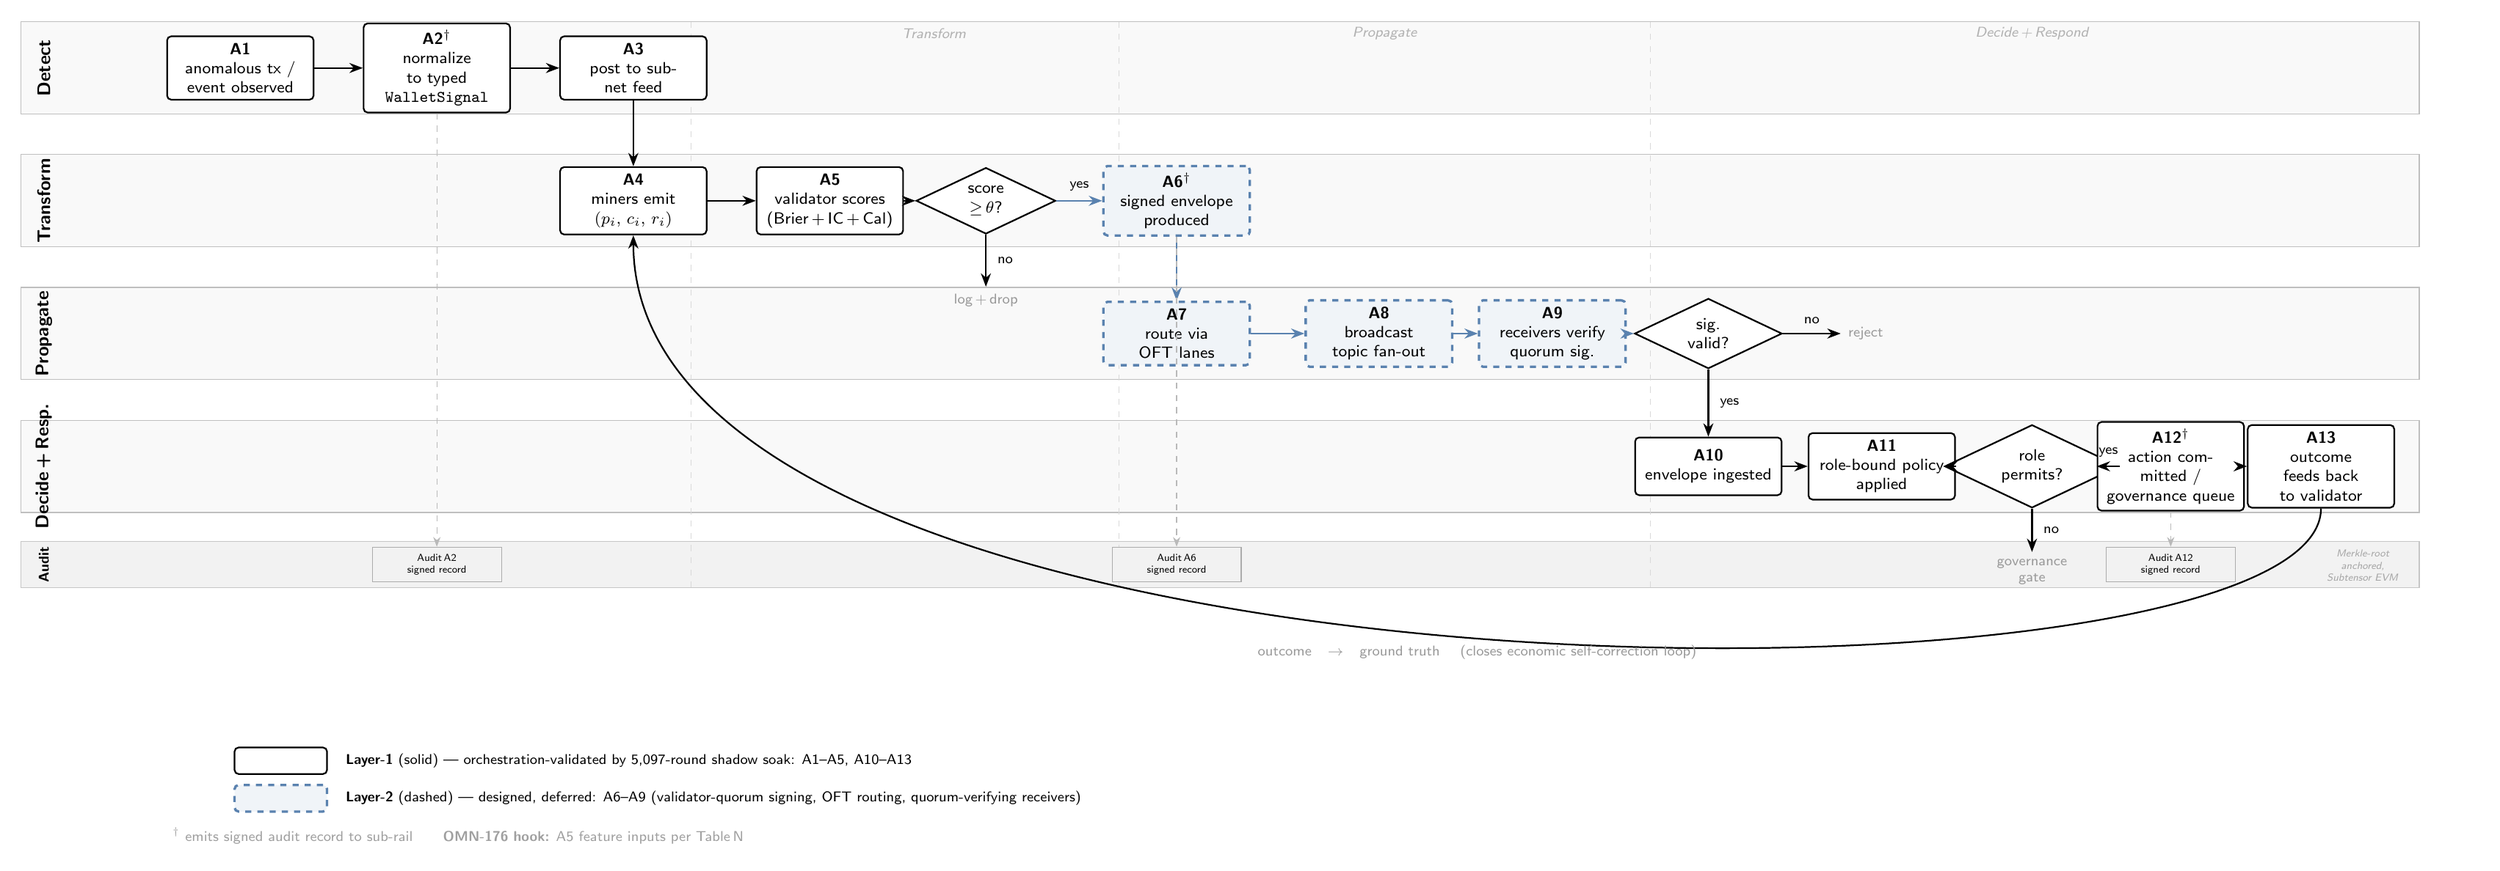
\begin{tikzpicture}[
  >=Stealth,
  every node/.style={align=center, font=\sffamily\footnotesize},
  %% L1 activity node (solid black border)
  act/.style={
    rectangle, rounded corners=2pt, draw=black, fill=white, thick,
    minimum width=2.5cm, minimum height=1.0cm, text width=2.3cm
  },
  %% L2 activity node (dashed layerblue border + tinted fill)
  actl2/.style={
    rectangle, rounded corners=2pt,
    draw=layerblue, dashed, line width=1.2pt,
    fill=layerblue!9,
    minimum width=2.5cm, minimum height=1.0cm, text width=2.3cm
  },
  %% Decision diamond
  dec/.style={
    diamond, aspect=2.1, draw=black, fill=white, thick,
    minimum width=2.1cm, minimum height=1.0cm
  },
  %% Audit record
  audrec/.style={
    rectangle, draw=gray!65, fill=gray!10, thin,
    minimum width=2.2cm, minimum height=0.5cm, text width=2.0cm,
    font=\sffamily\tiny
  },
  arr/.style={->, thick},
  arrl2/.style={->, thick, draw=layerblue},
]

%%====================================================================
%% COORDINATE PLAN (cm)
%%  Swimlanes are HORIZONTAL bands, time flows LEFT-TO-RIGHT.
%%
%%  Lane y-centres:
%%    Detect        y = 9.0   band: 8.2 -- 9.8
%%    Transform     y = 6.7   band: 5.9 -- 7.5
%%    Propagate     y = 4.4   band: 3.6 -- 5.2
%%    Decide+Resp   y = 2.1   band: 1.3 -- 2.9
%%    Audit         y = 0.4   band: 0.0 -- 0.8
%%
%%  Activity x-positions:
%%    A1=2.8  A2=6.2  A3=9.6
%%    A4=9.6  A5=13.0  D1=15.7  A6=19.0
%%    A7=19.0  A8=22.5  A9=25.5  D2=28.2
%%    A10=28.2  A11=31.2  D3=33.8  A12=36.2  A13=38.8
%%
%%  Canvas: x = -1.0 to 40.5,  y = -3.5 to 10.2
%%====================================================================

\pgfdeclarelayer{background}
\pgfsetlayers{background,main}

\begin{pgfonlayer}{background}
  %% Lane fills
  \fill[gray!5]  (-1.0,8.2) rectangle (40.5,9.8);
  \fill[gray!5]  (-1.0,5.9) rectangle (40.5,7.5);
  \fill[gray!5]  (-1.0,3.6) rectangle (40.5,5.2);
  \fill[gray!5]  (-1.0,1.3) rectangle (40.5,2.9);
  \fill[gray!10] (-1.0,0.0) rectangle (40.5,0.8);
  %% Lane borders
  \draw[gray!50,thin] (-1.0,8.2) rectangle (40.5,9.8);
  \draw[gray!50,thin] (-1.0,5.9) rectangle (40.5,7.5);
  \draw[gray!50,thin] (-1.0,3.6) rectangle (40.5,5.2);
  \draw[gray!50,thin] (-1.0,1.3) rectangle (40.5,2.9);
  \draw[gray!45,thin] (-1.0,0.0) rectangle (40.5,0.8);
  %% Phase dividers (light dashed verticals)
  \draw[gray!30,dashed,thin] (10.6,0.0) -- (10.6,9.8);
  \draw[gray!30,dashed,thin] (18.0,0.0) -- (18.0,9.8);
  \draw[gray!30,dashed,thin] (27.2,0.0) -- (27.2,9.8);
\end{pgfonlayer}

%% Phase header labels (italic, light)
\node[font=\sffamily\scriptsize\itshape,gray!60] at (5.7,9.6)  {Detect};
\node[font=\sffamily\scriptsize\itshape,gray!60] at (14.8,9.6) {Transform};
\node[font=\sffamily\scriptsize\itshape,gray!60] at (22.6,9.6) {Propagate};
\node[font=\sffamily\scriptsize\itshape,gray!60] at (33.8,9.6) {Decide\,+\,Respond};

%% Lane labels (bold, rotated on left)
\node[font=\sffamily\small\bfseries,rotate=90] at (-0.6,9.0)  {Detect};
\node[font=\sffamily\small\bfseries,rotate=90] at (-0.6,6.7)  {Transform};
\node[font=\sffamily\small\bfseries,rotate=90] at (-0.6,4.4)  {Propagate};
\node[font=\sffamily\small\bfseries,rotate=90,
      text width=2.5cm,align=center]             at (-0.6,2.1)  {Decide\,+\,Resp.};
\node[font=\sffamily\scriptsize\bfseries,rotate=90] at (-0.6,0.4) {Audit};

%%====================================================================
%% DETECT LANE  (L1: A1, A2, A3)
%%====================================================================
\node[act] (A1) at (2.8,9.0)
  {\textbf{A1}\\anomalous tx /\\event observed};

\node[act] (A2) at (6.2,9.0)
  {\textbf{A2}$^{\dagger}$\\normalize to typed \texttt{WalletSignal}};

\node[act] (A3) at (9.6,9.0)
  {\textbf{A3}\\post to subnet feed};

%%====================================================================
%% TRANSFORM LANE  (L1: A4, A5 | boundary D1 | L2: A6)
%%====================================================================
\node[act]   (A4) at (9.6,6.7)
  {\textbf{A4}\\miners emit\\$(p_i,\,c_i,\,r_i)$};

\node[act]   (A5) at (13.0,6.7)
  {\textbf{A5}\\validator scores\\(Brier\,+\,IC\,+\,Cal)};

\node[dec]   (D1) at (15.7,6.7)
  {score\\${\ge}\,\theta$?};

\node[actl2] (A6) at (19.0,6.7)
  {\textbf{A6}$^{\dagger}$\\signed envelope\\produced};

%%====================================================================
%% PROPAGATE LANE  (L2: A7, A8, A9 | D2)
%%====================================================================
\node[actl2] (A7) at (19.0,4.4)
  {\textbf{A7}\\route via\\OFT lanes};

\node[actl2] (A8) at (22.5,4.4)
  {\textbf{A8}\\broadcast\\topic fan-out};

\node[actl2] (A9) at (25.5,4.4)
  {\textbf{A9}\\receivers verify\\quorum sig.};

\node[dec]   (D2) at (28.2,4.4)
  {sig.\\valid?};

%%====================================================================
%% DECIDE + RESPOND LANE  (L1: A10-A13 | D3)
%%====================================================================
\node[act] (A10) at (28.2,2.1)
  {\textbf{A10}\\envelope ingested};

\node[act] (A11) at (31.2,2.1)
  {\textbf{A11}\\role-bound policy\\applied};

\node[dec] (D3)  at (33.8,2.1)
  {role\\permits?};

\node[act] (A12) at (36.2,2.1)
  {\textbf{A12}$^{\dagger}$\\action committed /\\governance queue};

\node[act] (A13) at (38.8,2.1)  {\textbf{A13}\\outcome feeds back\\to validator};

%%====================================================================
%% AUDIT SUB-RAIL
%%====================================================================
\node[audrec] (AUD2)  at (6.2,0.4)  {Audit\,A2\\signed record};
\node[audrec] (AUD6)  at (19.0,0.4) {Audit\,A6\\signed record};
\node[audrec] (AUD12) at (36.2,0.4) {Audit\,A12\\signed record};

\node[font=\sffamily\tiny,gray!70,anchor=west,text width=3.8cm]
  at (37.5,0.38) {\textit{Merkle-root\\anchored,\\Subtensor EVM}};

%%====================================================================
%% ARROWS — DETECT LANE
%%====================================================================
\draw[arr] (A1) -- (A2);
\draw[arr] (A2) -- (A3);

%%====================================================================
%% CROSS-LANE: A3 -> A4  (Detect -> Transform)
%%====================================================================
\draw[arr] (A3.south) -- (A4.north);

%%====================================================================
%% ARROWS — TRANSFORM LANE
%%====================================================================
\draw[arr] (A4) -- (A5);
\draw[arr] (A5) -- (D1);

%% D1 YES (score >= theta) -> A6  [L2 arrow, layerblue]
\draw[arrl2] (D1.east) --
  node[above,font=\sffamily\scriptsize,yshift=1pt] {yes}
  (A6.west);

%% D1 NO -> "log + drop" terminal (below D1)
\draw[arr] (D1.south) --
  node[right,font=\sffamily\scriptsize,xshift=2pt] {no}
  ++(0,-0.9)
  node[below,font=\sffamily\scriptsize,gray!80,text width=1.5cm]
  {log\,+\,drop};

%%====================================================================
%% CROSS-LANE: A6 -> A7  (Transform -> Propagate, both L2)
%%====================================================================
\draw[arrl2] (A6.south) -- (A7.north);

%%====================================================================
%% ARROWS — PROPAGATE LANE
%%====================================================================
\draw[arrl2] (A7) -- (A8);
\draw[arrl2] (A8) -- (A9);
\draw[arrl2] (A9) -- (D2);

%% D2 YES (sig valid) -> A10  (cross-lane, vertical down)
\draw[arr] (D2.south) --
  node[right,font=\sffamily\scriptsize,xshift=2pt] {yes}
  (A10.north);

%% D2 NO -> "reject" terminal (exit right)
\draw[arr] (D2.east) --
  node[above,font=\sffamily\scriptsize,yshift=1pt] {no}
  ++(1.0,0)
  node[right,font=\sffamily\scriptsize,gray!80] {reject};

%%====================================================================
%% ARROWS — DECIDE + RESPOND LANE
%%====================================================================
\draw[arr] (A10) -- (A11);
\draw[arr] (A11) -- (D3);

%% D3 YES (role permits) -> A12
\draw[arr] (D3.east) --
  node[above,font=\sffamily\scriptsize,yshift=1pt] {yes}
  (A12.west);

%% D3 NO -> "governance gate" terminal (below D3)
\draw[arr] (D3.south) --
  node[right,font=\sffamily\scriptsize,xshift=2pt] {no}
  ++(0,-0.75)
  node[below,font=\sffamily\scriptsize,gray!80,text width=2.2cm]
  {governance\\gate};

\draw[arr] (A12) -- (A13);

%%====================================================================
%% FEEDBACK LOOP: A13 -> A4  (curved arc below audit rail)
%%====================================================================
\draw[->,thick]
  (A13.south)
  .. controls (38.8,-2.4) and (9.6,-2.4)
  .. (A4.south)
  node[pos=0.5,below,font=\sffamily\scriptsize,gray!80,text width=9cm]
  {outcome $\;\to\;$ ground truth \quad(closes economic self-correction loop)};

%%====================================================================
%% AUDIT CONNECTORS  (thin dashed verticals from A2, A6, A12)
%%====================================================================
\draw[->,dashed,thin,gray!55] (A2.south)  -- (AUD2.north);
\draw[->,dashed,thin,gray!55] (A6.south)  -- (AUD6.north);
\draw[->,dashed,thin,gray!55] (A12.south) -- (AUD12.north);

%%====================================================================
%% LEGEND
%%====================================================================
\node[act,minimum width=1.6cm,minimum height=0.46cm,
      text width=1.4cm,inner sep=2pt,font=\sffamily\scriptsize]
  (LG1) at (3.5,-3.0) {};
\node[font=\sffamily\scriptsize,anchor=west] at (4.5,-3.0)
  {\textbf{Layer-1} (solid) --- orchestration-validated by
   5{,}097-round shadow soak: A1--A5, A10--A13};

\node[actl2,minimum width=1.6cm,minimum height=0.46cm,
      text width=1.4cm,inner sep=2pt,font=\sffamily\scriptsize]
  (LG2) at (3.5,-3.65) {};
\node[font=\sffamily\scriptsize,anchor=west] at (4.5,-3.65)
  {\textbf{Layer-2} (dashed) --- designed, deferred:
   A6--A9 (validator-quorum signing, OFT routing, quorum-verifying receivers)};

\node[font=\sffamily\scriptsize,gray!75,anchor=west] at (1.5,-4.3)
  {$^\dagger$ emits signed audit record to sub-rail%
  \quad\vrule width0pt height0pt\quad
  \textbf{OMN-176 hook:} A5 feature inputs per Table\,N};

\end{tikzpicture}%
}% end \sbox

\pdfpagewidth=\dimexpr\wd\figbox + 6pt\relax
\pdfpageheight=\dimexpr\ht\figbox + \dp\figbox + 6pt\relax
\hbox to \pdfpagewidth{\hss\usebox{\figbox}\hss}
\end{document}
